%!TEX root = main.tex
315 subjects from 19 countries participated in this study. Of the 315 test subjects, 112 (66 male / 46 female) finished the questionnaire. This corresponds to a completion rate of 40.79\%. The age of the subjects ranged from 19 to 46 with an average age of approximately 28 years. \par

\begin{table}[!ht]
	\centering
	\begin{tabu} spread 20pt {c c c c c }\toprule
	% & \multicolumn{6}{c}{Formulations}  \\ \cmidrule{2-7}
Total	&Male	&Female&	Experimental Group&	Control Group\\ \midrule
112     &	66  &	46 &	72                &	40\\
100.00\%& 58.93\%&	41.07\%&	64.29\%&	35.71\%\\ \bottomrule
	\end{tabu}
	\caption{Random sample of the participants before the adjustment distinguished by ‘gender’ and experimental / control group.}
	\label{tab:gender}
\end{table}
However, due to significant mistakes and deviation of the average and anticipated perfor-mance time, the participants’ number was adjusted to a total of 86.  \par
The experiment was based on a two factorial between the distinguishing mark (depletion and non-depletion) designs. The main dependent measure was social risk in decision-making. The decision-making served as a measurement of social risk tendencies. The adjusted sample consisted of (N = 86) participants (33 male / 53 female) aged between 20 and 46 (M = 28.151; SD = 5.13). The experimental group consisted of (N = 30) participants  (13 male / 17 female) and the control group consisted of (N = 56) participants (20 male / 36 female).\par
The experiment was designed as an online questionnaire study. Its first aim was to provide the participants with the opportunity for self-evaluation in the context of consumer, spending and risk behaviour. After answering the self-evaluation part, the participants were randomly assigned to two groups. Group 1 (experimental group) had to accomplish a ‘Stroop test’, containing three sets of 60 questions each. The experimental-condition task was designed to de-plete participants within approximately 15 to 20 minutes. The task used for the control group was identical to the one used in the experimental condition but did not include the depletion measure. Therefore, all words were presented in dark grey (see above), so that a depletion of the control group was not expected. After completing the task, participants were instructed to decide between two alternatives of a product, which could be distinguished by one attribute only (e.g. colour). Figure \ref{fig:os_product_choice} depicts an example of the decision making task of the questionnaire. \par

\begin{figure}[h!]
\center
	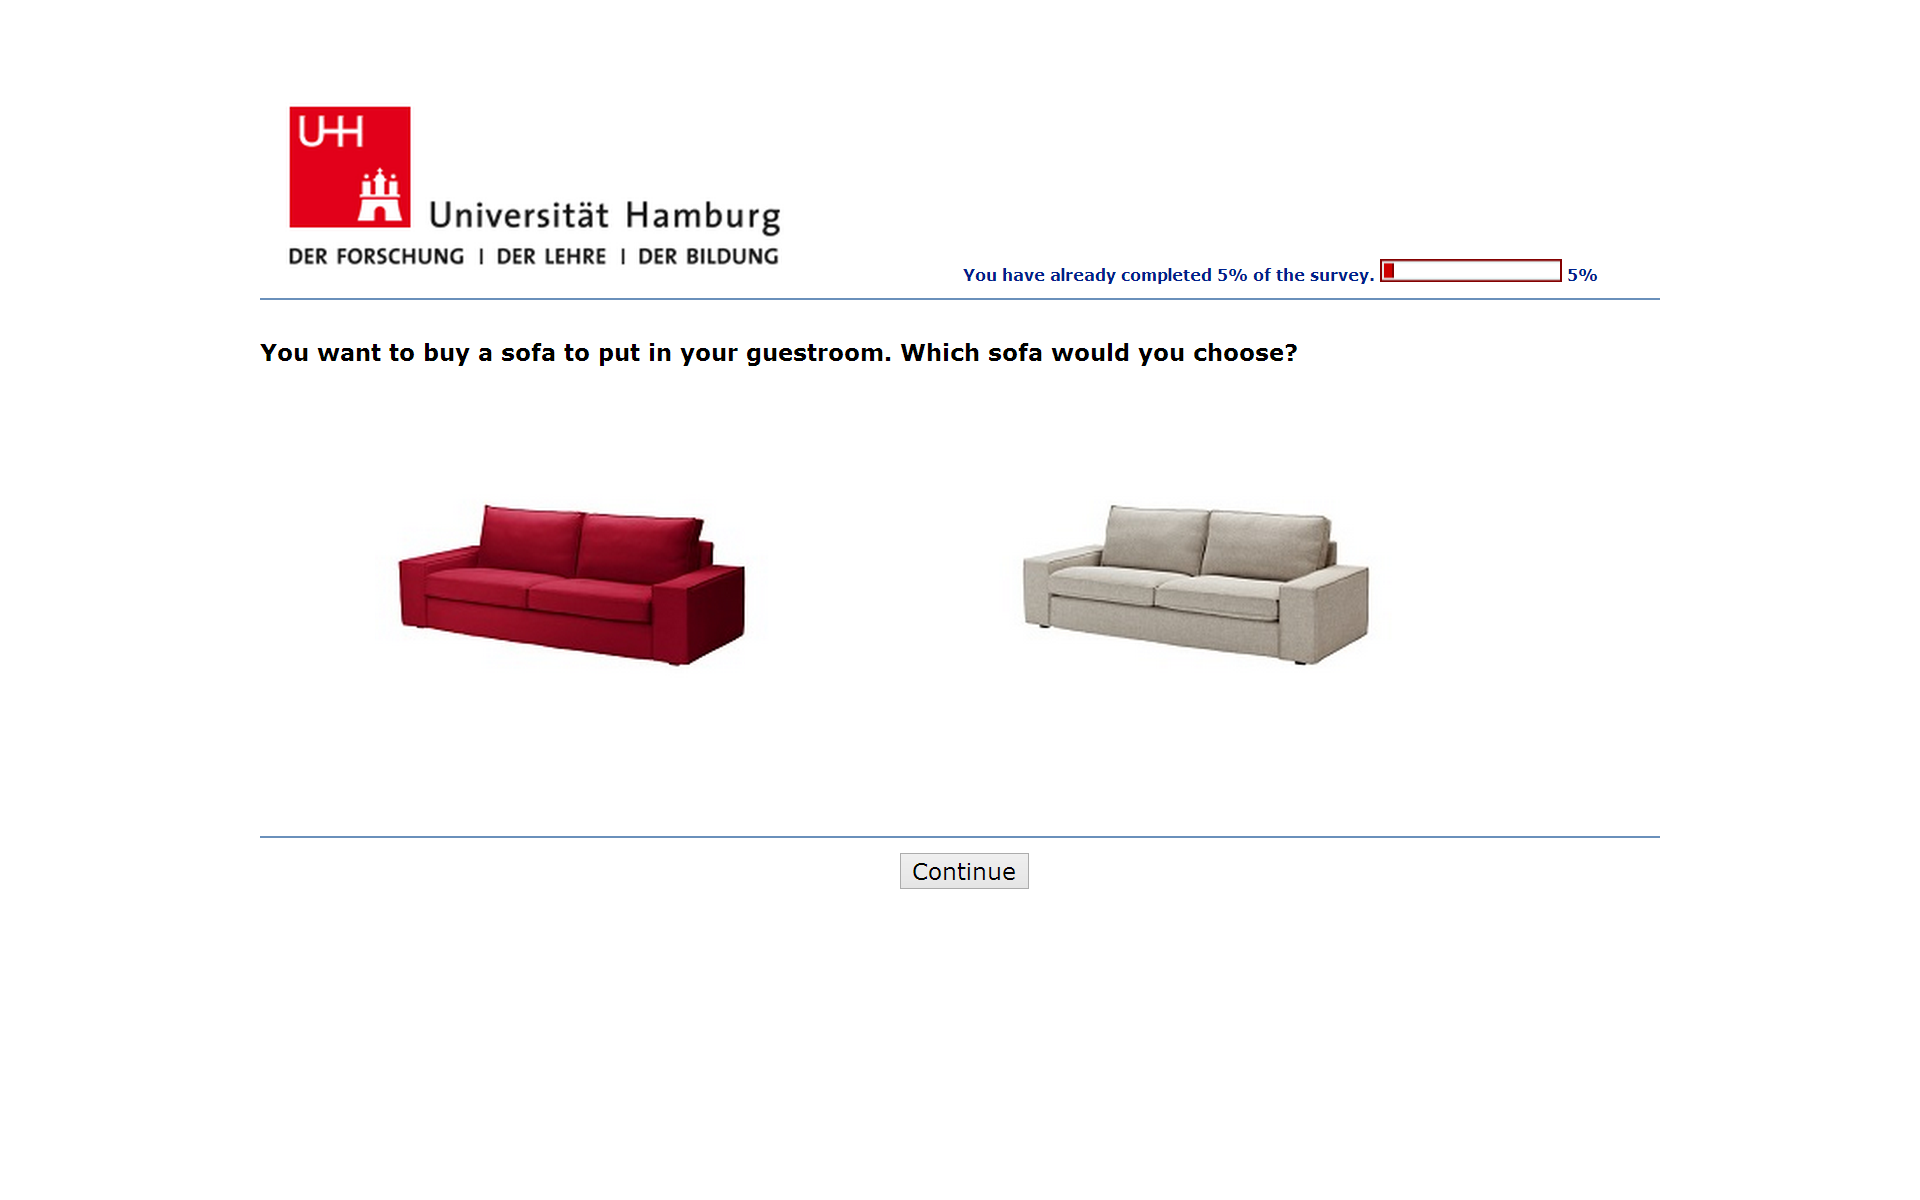
\includegraphics[width=0.9\textwidth]{images/os_product_choice.png}
  \caption{Example of product choice in online questionnaire (sofa)}\label{fig:os_product_choice}
\end{figure}
By putting the decision in a situation of a social context ‘You want to buy a sofa to put in your guestroom’, we tried to emphasize the social contribution ‘people will see this item that I bought and might judge me on the basis of this purchase’. Each product was placed in a dif-ferent social framework\footnote{In order not to violate any trademark rights, the brands in the online questionnaire have been removed. Howev-er, some of the products posses a high recognition factor and might influence the participants after all.}. After the decision-making task based on purchases the questionnaire proceeded with questions based on the judges’ dilemma (compare Chapter \ref{sec:consumerchoice}). Before the participants could finalize their decision they were informed that their verdict as to whether the perpetrator would be granted probation or if he/she would remain in custody was crucial. They were also asked to keep in mind that while resocialization is an important objective, so is keeping in custody a possible repeater. Both tasks regarding decision-making were aimed at generating an environment of social risk. After the decision-making task participants were instructed to answer questions in order to examine the degree of their depletion (see Chapter \ref{sec:consumerchoice}). Subsequently participants were asked to state their perceived level of exhaustion on a Likert scale (ranging from ‘not at all exhausted’ to ‘very exhausted’) and how they assessed the level of difficulty regarding the Stroop test (ranging from ‘very easy’ to ‘very difficult’).